\documentclass[12pt,a4paper]{article}
\usepackage[utf8]{inputenc}
\usepackage{amsmath}
\usepackage{amssymb}
\usepackage{geometry}
\usepackage{graphicx}

\geometry{margin=2.5cm}

\title{\textbf{Preparatório - Ensino Integrado IFPE}}
\author{20/05/2025}
\date{\vspace{-5ex}}


\begin{document}

\maketitle

\textbf{\begin{center}
    Professor: Rogério Tiúma
\end{center}}

\section*{Prova 2020.1 - PROEJA}


1. O Sr. João percebeu que uma torneira, no quintal da sua casa, estava com um pequeno vazamento. O neto
dele, Gabriel, observou que a torneira gotejava 10 vezes a cada 20 segundos. Utilizando uma seringa
plástica, Gabriel concluiu que as gotas sempre tinham o volume igual a 0,4 ml. Em um intervalo de 2
horas, até consertar a torneira, quantos mililitros de água foram desperdiçados no total? 

\vspace{2ex}

a) 1.400 ml
b) 1.420 ml
c) 1.480 ml
d) 1.460 ml
e) 1.440 ml 

\vspace{2ex}

2. Eugênio é professor de Matemática da Educação de Jovens e Adultos, em uma escola municipal. Ele tem
por hábito, nas sextas-feiras, apresentar um desafio para os seus alunos. Na última sexta-feira, o desafio
foi: 

\vspace{2ex}
“No quadrado da FIGURA 1, troque as letras por números inteiros de tal forma que as somas dos
números inteiros das linhas, das colunas e das diagonais sejam iguais”. 
\vspace{2ex}

\begin{figure}[h]
\centering
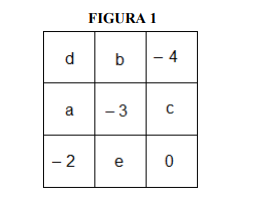
\includegraphics[width=0.3 \linewidth]{./figuras/Fig.png}
\end{figure}

Carlos, sentindo-se motivado pela tarefa, fez alguns cálculos e apresentou a sua solução. Supondo que
Carlos tenha acertado o desafio, a soma a + b + c + d + e é igual a 

\vspace{2ex}
a) – 15.
b) – 17.
c) – 18.
d) – 13.
e) – 12. 
\vspace{2ex}

3. O Vaticano é um país reconhecido pela Organização das Nações Unidas (ONU). Situado na zona norte
da cidade de Roma, é considerado o menor país do mundo, com 0,45 $km^2$ de extensão. Se o Vaticano tivesse a forma de um círculo, qual seria a medida do quadrado de seu raio? (Utilize a aproximação $\pi$ = 3.) 

\vspace{2ex}
a) 0,13 km
b) 0,14 km
c) 0,15 km
d) 0,16 km
e) 0,17 km 
\vspace{2ex}

4. O Sr. José tem um escritório de contabilidade, onde trabalham 20 pessoas com vários graus de
escolaridade diferentes. Sua neta, Ana, terminou o Curso de Ciências Contábeis e vai ser sócia do avô no
escritório. O Sr. José apresentou à neta a seguinte tabela com a distribuição dos salários dos funcionários. 

\begin{figure}[ht]
\centering
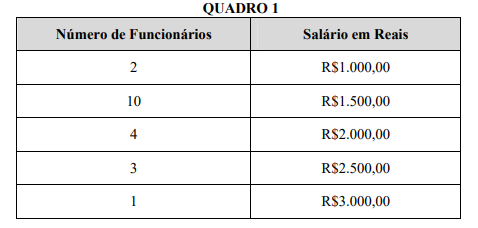
\includegraphics[width=0.6 \linewidth]{./figuras/quadro1.png}
\end{figure}

Com os dados disponíveis no QUADRO 1, conclui-se que o salário médio do escritório é

\vspace{2ex}
a) R\$1.475,00.
b) R\$1.775,00.
c) R\$1.675,00.
d) R\$1.575,00.
e) R\$1.875,00.

\vspace{2ex}

5. O Sr. Otaviano resgatou R\$67.500,00, saldo referente à sua aplicação em títulos de capitalização. Ele
decidiu dividir essa quantia em partes diretamente proporcionais às idades de seus netos, Valdson,
Mônica, Jansen, Ana e Sônia, as quais são, respectivamente, 24, 21, 20, 18 e 7. Aplicada essa divisão
do dinheiro, é CORRETO afirmar que

\vspace{2ex}
a) Jansen recebeu R\$15.000,00.
b) Valdson recebeu R\$19.000,00.
c) Sônia recebeu R\$4.250,00.
d) Mônica recebeu R\$17.500,00.
e) Ana recebeu R\$13.250,00. 

\vspace{2ex}

6. O Sr. Fernando comprou um terreno retangular que mede 18 metros de largura por 30 metros de
comprimento. Para cercar completamente sua propriedade, ele comprou estacas de madeira e rolos de
arame farpado. A pessoa contratada para fazer o serviço sugeriu que fossem colocados cinco fios de arame
contornando todo o perímetro, conforme a FIGURA 2.

\begin{figure}[ht]
\centering
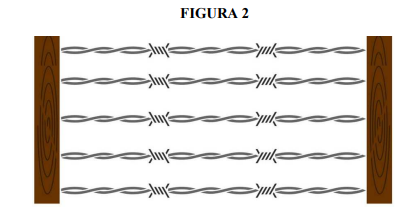
\includegraphics[width=0.6 \linewidth]{./figuras/Fig2.png}
\end{figure}

Fernando acatou a sugestão. Sabendo que o arame farpado é vendido em rolos de 50 metros, determine
quantos rolos, no mínimo, serão comprados. 

\vspace{2ex}
a) 13.
b) 12.
c) 11.
d) 9.
e) 10. 
\vspace{2ex}

7. André estava esperando a condução escolar quando percebeu que, pela posição do sol, um poste projetava
uma sombra de comprimento “x”, conforme a FIGURA 3. Pesquisando na internet, ele descobriu que
aquele tipo de poste tinha 10 metros de altura. Como ele estava estudando Trigonometria na escola, tentou
descobrir o comprimento da sombra (representado pela letra “x”), o qual é de, aproximadamente,
(Dados: Tg $\alpha$ = 0,75) 

\begin{figure}[ht]
\centering
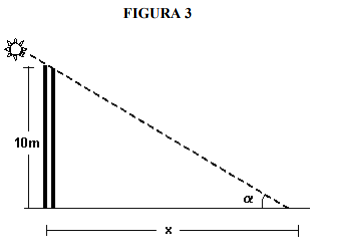
\includegraphics[width=0.6 \linewidth]{./figuras/Fig3.png}
\end{figure}

\vspace{2ex}
a) 17 metros.
b) 16 metros.
c) 13 metros.
d) 14 metros.
e) 15 metros. 
\vspace{2ex}

8. Em determinado ano, as moedas de R\$0,25 tinham, numa de suas faces, um polígono regular com 7 lados,
como se pode ver na FIGURA 4.

\begin{figure}[ht]
\centering
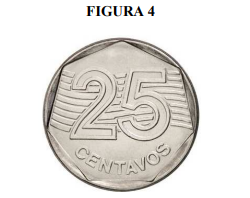
\includegraphics[width=0.3 \linewidth]{./figuras/Fig4.png}
\end{figure}

Quanto vale a soma dos ângulos internos desse polígono de 7 lados?

\vspace{2ex}
a) 1.160°
b) 900°
c) 1.180°
d) 1.260°
e) 1.620°
\vspace{2ex}



9. Na tentativa de incentivar os alunos da Educação de Jovens e Adultos do Ensino Fundamental II, a
Coordenação criou uma gincana em que os estudantes respondiam a perguntas sobre vários assuntos.
Numa dessas rodadas da gincana, o professor de Matemática propôs a seguinte pergunta:

\vspace{2ex}
“Ao quadrado de um número x, você adiciona 7 e obtém sete vezes o
número x, menos 3. Quais são as raízes dessa equação?”
A resposta CORRETA desse problema é

\vspace{2ex}
a) 2 e – 5.
b) – 2 e – 5.
c) – 2 e 5.
d) 2 e 5.
e) a equação não tem raiz real.
\vspace{2ex}

10. Três amigas, Ana, Simone e Marília, resolveram abrir uma loja para vender roupas e bolsas. Elas
procuraram um especialista para obter informações sobre como tabelar os preços de suas mercadorias. O
especialista informou o seguinte:

\vspace{2ex}
\begin{enumerate}
\item se a venda fosse em dinheiro, o valor da mercadoria deveria ser aumentado em 30\% em relação ao
preço de compra, que é a chamada margem de lucro.
\item se a venda fosse em cartão de débito, após o aumento de 30\%, elas deveriam acrescentar a taxa de 3%
cobrada pela administradora da máquina.
\item se a venda fosse em cartão de crédito, após o aumento de 30\%, elas deveriam acrescentar a taxa de 5%
cobrada pela administradora da máquina.
Então, se elas compraram uma bolsa por R\$120,00, qual deve ser o preço dessa bolsa para uma venda no
cartão de crédito?
\end{enumerate}
\vspace{2ex}

a) R\$163,80
b) R\$161,80
c) R\$162,80
d) R\$160,80
e) R\$164,80 

\subsection*{Gabarito}

1. E // 2. C // 3. C // 4. B // 5. A // 6. E // 7. C // 8. B // 19. D // 20.  A

\end{document}